
%see https://tex.stackexchange.com/questions/25798/how-can-i-add-abstract-and-acknowledgement-pages-into-the-table-of-contents
\chapter*{Curriculum Vitae}%
\addcontentsline{toc}{chapter}{Curriculum Vitae}%

\begin{wrapfigure}{l}{0.28\linewidth}
\centering
\vspace{-4.0mm}
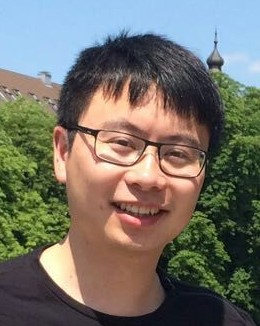
\includegraphics[width=\linewidth]{images/peng_4x3.jpg}
\end{wrapfigure}

Dongliang Peng was born on October 26, 1987 
in Yonghe, Liuyang, Changsha, Hunan, China.
In 2009, he obtained his bachelor's degree in Mapping Engineering
at Central South University (CSU), Changsha, China.
His bachelor's thesis is entitled 
``Updating Geographical Data based on AutoCAD''.
He continued to study 
Cartography and Geographic Information Engineering at CSU.
In 2012, he obtained his master's degree with thesis 
``A Methodology of Morphing Transformation of Linear Features
for Map Continuous Generalization''.
Both the bachelor's and master's theses 
were under the supervision of Prof.\ Dr.\ Min Deng.
From 2012 to 2017, he pursued his Ph.D.\ degree in Computer Science
at Julius Maximilian University of Würzburg (JMU), Germany.
The title of his dissertation is
``An Optimization-Based Approach for Continuous Map Generalization'',
which was supervised by
Prof.\ Dr.\ Alexander Wolff and Prof.\ Dr.\ Jan-Henrik Haunert.


Since 2018, he became a postdoctoral researcher
in Section of GIS Technology,
Delft University of Technology (TU Delft), The Netherlands.
He works with Prof.\ Dr.\ Peter van Oosterom and
Dr.\ Martijn Meijers on the topic of vario-scale maps. 



